% §6 The scale evolution in generator form --- blueprint chapter 11
% (blueprint/src/parts/11-generator.tex), statements and proofs of record verbatim. Drafted
% 2026-09-15; prose rewritten 2026-09-18 at the author's review (scripts/splice-prose.py, the
% statements and proofs untouched): the section opens from what its reader knows, scale space
% as an equation, says what the generator is and why the kind of operator matters, and maps its
% three statements; the intuition comes before each statement and the comments on a statement or
% its proof after it; the Lean and Mathlib talk is gone from the body (what it said about the
% fractional Laplacian and the class of g in clause (4) is kept as mathematics); a schematic
% figure of the generator as a superposition of second differences (fig-generator.tex).
%
% Contents and departures from the blueprint chapter:
%   - all three nodes transcribed under their markers: def:signal-class, prop:scale-evolution,
%     prop:corner-generators; what is machine-checked and on what is section 1.1's to say, and
%     the body deliberately does not (the Thorin clause of the corner generators uses ledger A3
%     through chapter 10's representation; the rest of the chapter rests on Lean core);
%   - the blueprint's status annotations are not transcribed; what a reader needs from them is
%     said in prose: which class the signal-side identity is stated on and why, that both
%     derivative clauses name their derivative, how clause (2) of the corner generators is
%     formalised (at the symbol and the jump measure, Mathlib having no fractional Laplacian),
%     the class of g in clause (4), and the Duits et al. anchor for the alpha-scale-space
%     equation (R116);
%   - the chapter's pointer to the locality chapter (module C) becomes a sentence naming the
%     next module's subject without promising it (hub RELEASES.md rule 1);
%   - rem:causal-relation-generator is paper-only, this section's one relation-to-the-causal-
%     theory remark (ADR-0003), from the blueprint's twin comment on prop:scale-evolution;
%   - the infinitesimal theory beyond the generator form (the scale-Cauchy problem, the atomic
%     generators, Phillips' formula) is outside this paper, as the blueprint's header says, and
%     the section says so where the question arises.

\section{The scale evolution in generator form}\label{sec:generator}

Linear scale space is usually met as an equation: the scale space of a signal is the solution
of the heat equation with the signal as initial value, and the kernel is what solving the
equation produces. The classification of the line paper runs the other way. It is stated on
the kernels, and it says nothing about what equation, if any, a member of the class solves.
This section supplies the equation. For every admissible family, in its canonical gauge, the
scale space $u(t,x)$ of a Schwartz signal satisfies
\[
  \partial_t u = \mathcal{A}_t u ,
\]
with a generator $\mathcal{A}_t$ that is read off the pair $(a,k)$. The Gaussian coefficient
contributes a second derivative. The profile contributes, for every displacement size, the
amount by which the average of the signal's two neighbours at that distance exceeds the signal
(Figure~\ref{fig:generator}). After a reparametrization of scale this is the heat equation for
the Gaussian and the fractional heat equation of the $\alpha$-scale spaces for the stable
family, so the classical equations are recovered. The other members have equations of their
own. The generator of the \Matern{} family is a \emph{bounded} operator, which is how its
exact implementation (\S\ref{sec:implementation}) looks at the level of the generator. The
generator of a $\Cin$ ray is a single second difference.

The equation matters for a second reason. Locality of the evolution and the non-creation of
local extrema are the requirements from which the Gaussian axiomatics select one member
(\sscite{koenderink1984structure}; \sscite{lindeberg2011generalized}). They are conditions on
the evolution in scale, and this is the form in which they are asked. They are the subject of
the next module. The present section states the form and computes the generators of the
corners, and stops there. The rest of the infinitesimal theory is outside this paper: the
existence and uniqueness of solutions of the evolution equation, the decomposition of a
generator over the generators of the extreme rays of \S\ref{sec:cone}, and the infinitesimal
form of the bridge of \S\ref{sec:bridge}.

The signals are taken in the Schwartz class. It is the simplest choice that makes every step
of the evolution identity unconditional. Enlarging it is a question this paper does not
answer: to the Sobolev class $W^{2,1}$, two derivatives in $\Lone$, for the Gaussian part, or
to the full domain of the generator in general.

% shared with blueprint def:signal-class
\begin{definition}[the signal class]\label{def:signal-class}
$\mathcal{D} := \Sch$ is the Schwartz class on the line: smooth functions all of whose
derivatives decay faster than every polynomial. It is contained in $\Lone$, is stable under
differentiation, and its Fourier image is itself.
\end{definition}

The equation is simplest on the Fourier side. In the canonical gauge the kernel at scale $t$
has transform $e^{-F(t\omega)}$, and differentiating in $t$ brings down the symbol
$B = \omega F'$ of \ref{eq:symbol}, evaluated at $t\omega$ and divided by $t$. Since
$B \ge 0$, every wavenumber is damped, at the rate $B(t\omega)/t$. The symbol is a classical
object of the probability literature. A self-decomposable law is the limit law of a process of
Ornstein--Uhlenbeck type, its exponent being $\int_0^\infty \psi(e^{-s}\omega)\,ds$ for the
exponent $\psi$ of a \Levy{} process, the background driving process, written with the sign of
this paper, so that the process at time $1$ has the transform $e^{-\psi}$
(\sscite{sato1999levy}, Theorem~17.5, pp.~108--109), and differentiating that representation
gives $\psi = \omega F' = B$. What this section adds to it is the reading as an evolution
equation for the signal, with its domain and its constants. The signal side is the same
identity read through the displacement dictionary of
Remark~\ref{rem:displacement-dictionary}. Here $\omega^2$ is the symbol of $-\partial_x^2$, and
$1 - \cos(\omega h)$ is the symbol of $g \mapsto g - \tfrac12(g(\cdot - h) + g(\cdot + h))$,
the negative of the symmetric second difference at distance $h$. So the two terms of $B$
become a Laplacian and a superposition of second differences over the displacement sizes. The
differences are weighted by the tail measure $\varpi$ and dilated to the current scale.
The factor $t^{-1}$ says that the natural clock is log-scale: in $\theta = \log t$ the
generators at different scales are dilates of one operator.

% Figure: the generator as a superposition of symmetric second differences. Referenced from
% section 6 before prop:scale-evolution. Pure TikZ, schematic (2026-09-18, the author's review:
% illustrate where a schematic carries the point). Three panels: a Cin ray (one displacement
% size), the Matern member (every size, exponential weights), a stable member (every size,
% power-law weights). Line width stands for the weight varpi(dv) of the size; nothing is to scale.

\begin{figure}[t]
\centering
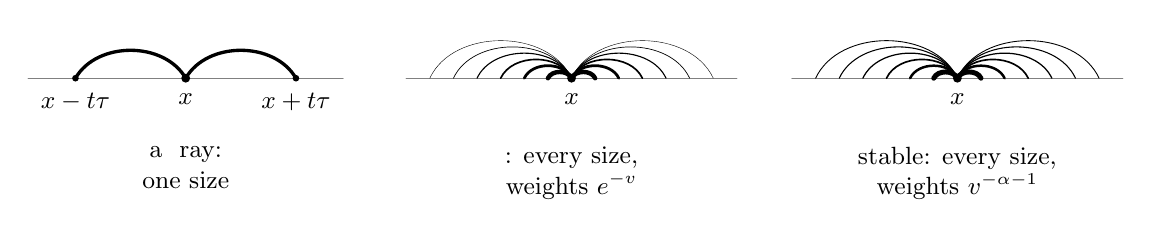
\begin{tikzpicture}[every node/.style={font=\small}, line cap=round, >=stealth]

% --- panel (a): a Cin ray ---------------------------------------------------------------
\begin{scope}[shift={(0,0)}]
\draw[gray] (-2.0,0) -- (2.0,0);
\fill (0,0) circle (1.6pt) node[below=2pt] {$x$};
\draw[line width=1.2pt] (0,0) to[out=60,in=120] (1.4,0);
\draw[line width=1.2pt] (0,0) to[out=120,in=60] (-1.4,0);
\fill (1.4,0) circle (1.2pt) node[below=2pt] {$x + t\tau$};
\fill (-1.4,0) circle (1.2pt) node[below=2pt] {$x - t\tau$};
\node[anchor=north, align=center] at (0,-0.75) {a $\Cin$ ray:\\ one size};
\end{scope}

% --- panel (b): the Matern member ---------------------------------------------------------
\begin{scope}[shift={(4.9,0)}]
\draw[gray] (-2.1,0) -- (2.1,0);
\fill (0,0) circle (1.6pt) node[below=2pt] {$x$};
\foreach \d/\w in {0.3/1.6, 0.6/1.0, 0.9/0.6, 1.2/0.4, 1.5/0.25, 1.8/0.15} {
  \draw[line width=\w pt] (0,0) to[out=65,in=115] (\d,0);
  \draw[line width=\w pt] (0,0) to[out=115,in=65] (-\d,0);
}
\node[anchor=north, align=center] at (0,-0.75) {\Matern{}: every size,\\ weights $e^{-v}$};
\end{scope}

% --- panel (c): a stable member -------------------------------------------------------------
\begin{scope}[shift={(9.8,0)}]
\draw[gray] (-2.1,0) -- (2.1,0);
\fill (0,0) circle (1.6pt) node[below=2pt] {$x$};
\foreach \d/\w in {0.3/1.8, 0.6/0.9, 0.9/0.6, 1.2/0.45, 1.5/0.38, 1.8/0.32} {
  \draw[line width=\w pt] (0,0) to[out=65,in=115] (\d,0);
  \draw[line width=\w pt] (0,0) to[out=115,in=65] (-\d,0);
}
\node[anchor=north, align=center] at (0,-0.75) {stable: every size,\\ weights $v^{-\alpha-1}$};
\end{scope}

\end{tikzpicture}
\caption{The jump part of the generator \ref{eq:evolution-signal}, schematically. At a
position $x$ and a scale $t$ the generator compares $g(x)$ with the average of its two
neighbours at distance $tv$, for every displacement size $v$. It sums the differences with the
weight $\varpi(dv)$, drawn here as line width. A $\Cin$ ray has one size, so its generator is a
single second difference. The \Matern{} member has every size with exponentially decaying
weight, and the sum is a bounded operator, $2\gamma/t$ times the difference between
convolution by the Laplace kernel of range $t$ and the identity. A stable member has every
size with power-law weight, not summable at small sizes, and the sum is the fractional
Laplacian. The Gaussian part of a generator is not drawn: it is the limit of the same
comparison at vanishing size, a multiple of the second derivative.}
\label{fig:generator}
\end{figure}


% shared with blueprint prop:scale-evolution
\begin{proposition}[the scale evolution in generator form]\label{prop:scale-evolution}
Let $F$ be admissible with data $(a,k)$ and $\varpi = -dk$, and let $u(t,\cdot) :=
\mu_{0,t} * f$ be the scale space of $f \in \mathcal{D}$ in the canonical gauge. Then on the
Fourier side
\begin{equation}\label{eq:evolution-fourier}
  \partial_t\hat u(t,\omega) = -\frac1t\,B(t\omega)\,\hat u(t,\omega),
  \qquad
  B(\omega) = \omega F'(\omega)
   = 2a\,\omega^2 + \int_{(0,\infty)}\bigl(1 - \cos\omega v\bigr)\,\varpi(dv),
\end{equation}
for every $\omega$ and every $t > 0$, and on the signal side
\begin{equation}\label{eq:evolution-signal}
  \partial_t u(t,x) = \mathcal{A}_t u(t,x),
  \qquad
  \mathcal{A}_t g(x) := 2at\,g''(x)
   - \frac1t\int_{(0,\infty)}\Bigl[g(x) - \tfrac12\bigl(g(x-tv) + g(x+tv)\bigr)\Bigr]\,\varpi(dv),
\end{equation}
the integral converging absolutely for $g \in \mathcal{D}$. The generators at different scales
are conjugate, $\mathcal{A}_t = t^{-1}\Dil{t}\,\mathcal{A}_1\,\Dil{t}^{-1}$, with
$\mathcal{A}_1 = -B(D)$ and $D = -i\partial_x$; in log-scale $\theta = \log t$ the
evolution reads $\partial_\theta u = \Dil{t}\mathcal{A}_1\Dil{t}^{-1}u$.
\end{proposition}

The operator $\mathcal{A}_1 = -B(D)$ is the generator of the symmetric \Levy{} process with
Gaussian part $2a$ and folded jump measure $\varpi$, which is the probabilistic reading of the
symbol and is used nowhere below.

The signal-side identity is a pointwise derivative in the scale at a fixed position. Its
right-hand side contains a second space derivative of the scale space. That derivative
exists: the scale space of a Schwartz signal is twice differentiable. The one step of the proof that
is not a computation on symbols comes from the tails. The scale space $u(t,\cdot)$ is not a
Schwartz function, since it inherits the tails of the kernel, and those are polynomial for the
Student-t and stable families. So the generator is first moved off $u$ and onto the signal,
by translation invariance, and the multiplier identity is applied there.

\begin{proof}
$\hat u(t,\omega) = e^{-F(t\omega)}\hat f(\omega)$, and $F$ is $C^1$ off the origin with
$\omega F'(\omega) = B(\omega)$ by Lemma~\ref{lem:selfdecomposable-exponents} and
\ref{eq:symbol}; differentiating in $t$ gives \ref{eq:evolution-fourier}, since
$\partial_t F(t\omega) = \omega F'(t\omega) = t^{-1}B(t\omega)$.

For \ref{eq:evolution-signal}: $B(t\omega) = 2at^2\omega^2 + \int(1 - \cos t\omega
v)\,\varpi(dv)$, where $\omega^2$ is the symbol of $-\partial_x^2$ and $1 - \cos(\omega\,tv)$
is the symbol of $g \mapsto g - \tfrac12(\Tr{tv} + \Tr{-tv})g$. So the Fourier multiplier
$B(tD)$ acts on $g \in \mathcal{D}$ as
$-2at^2g'' + \int[g - \tfrac12(g(\cdot - tv) + g(\cdot + tv))]\,\varpi(dv)$, the integrand
being bounded by $\min(2\|g\|_\infty, \tfrac12t^2v^2\|g''\|_\infty)$ and hence
$\varpi$-integrable, since $\int (1 \wedge v^2)\,\varpi < \infty$. Thus
$\mathcal{A}_t = -t^{-1}B(tD)$ on $\mathcal{D}$, which is \ref{eq:evolution-signal} read as a
Fourier multiplier.

That $\partial_t u$ equals $\mathcal{A}_tu$ pointwise is the inverse transform of
\ref{eq:evolution-fourier}, and the inversion is used twice. Write
$\langle\kappa_\varphi, h\rangle = \int_\RR h(z)\cos(\omega z - \varphi)\,dz$ for the pairing of
$h$ with the character of frequency $\omega$ and phase $\varphi$. For a symmetric probability
measure $\nu$ and an $h$ that is continuous and integrable with integrable transform,
\[
  (\nu * h)(x) \;=\; \frac{1}{2\pi}\int_\RR \hat\nu(\omega)\,
    \langle\kappa_{\omega x}, h\rangle\,d\omega ,
\]
by Fourier inversion for $h$ together with one exchange of integrals against the finite $\nu$;
the symmetry of $\nu$ is what turns the $\nu$-average of $\cos(\omega(x-y))$ into
$\hat\nu(\omega)\cos(\omega x)$, and no other step of the proof uses it.

Read at $h = f$ and $\nu = \mu_{0,s}$, this represents the scale space as
$u(s,x) = (2\pi)^{-1}\int e^{-F(s\omega)}\langle\kappa_{\omega x},f\rangle\,d\omega$.
Differentiating under that integral at $s = t$ is licensed on $s \in (t/2, 3t/2)$ by the
dominating function $s^{-1}B(s\omega)\,|\langle\kappa_{\omega x},f\rangle|$, which is integrable
because $B(s\omega) \le C(1 + s^2\omega^2)$ by Lemma~\ref{lem:quadratic-growth} while
$|\langle\kappa_\varphi, f\rangle| \le (\|f\|_1 + \|f''\|_1)/(1 + \omega^2)$ uniformly in the
phase --- the two crude bounds $|\langle\kappa_\varphi,f\rangle| \le \|f\|_1$ and
$\omega^2|\langle\kappa_\varphi,f\rangle| = |\langle\kappa_\varphi,f''\rangle| \le \|f''\|_1$,
combined --- and iterating that estimate on $f''$ improves the decay to
$(1 + \omega^2)^{-2}$, which is one power more than the symbol's growth consumes. So
$\partial_tu(t,x)
 = -(2\pi)^{-1}\int t^{-1}B(t\omega)e^{-F(t\omega)}\langle\kappa_{\omega x},f\rangle\,d\omega$.

Read at $h = \mathcal{A}_tf$ and $\nu = \mu_{0,t}$, it represents the right-hand side --- but
only after the generator has been moved off $u(t,\cdot)$, which is \emph{not} in $\mathcal{D}$:
the scale space inherits the kernel's tails, and the Student-t and stable kernels have
polynomial ones, so the multiplier identity above does not
apply to it. Translation invariance supplies the step: $\mathcal{A}_t$ commutes with convolution
by a finite measure, $\mathcal{A}_t(\nu * f) = \nu * (\mathcal{A}_tf)$, the exchange of the
$\varpi$-integral with the $\nu$-integral being licensed by the same bound
$\min(2\|f\|_\infty, \tfrac12t^2v^2\|f''\|_\infty)$ that makes the generator's own integral
converge. Hence $\mathcal{A}_tu(t,\cdot) = \mu_{0,t} * (\mathcal{A}_tf)$, whose argument is
continuous and integrable, and
$\langle\kappa_{\omega x},\mathcal{A}_tf\rangle = -t^{-1}B(t\omega)\langle\kappa_{\omega x},f\rangle$
by the multiplier identity at the scale $t$. The two frequency integrands agree, which is
\ref{eq:evolution-signal}.

Conjugation: $\Dil{t}$ has symbol map $\omega \mapsto t\omega$, so
$\Dil{t}B(D)\Dil{t}^{-1} = B(tD)$; and $\partial_\theta = t\partial_t$.
\end{proof}

\begin{remark}[relation to the causal theory]\label{rem:causal-relation-generator}
The causal article \sscite{fagerstrom2026hemigroup} states its scale evolution in the same
form. In place of the multiplier identity it uses Phillips' formula, which gives the generator
of a subordinated semigroup from that of the original one (\sscite{schilling2012bernstein},
Chapter~13). The causal generator carries the memory kernel of the half-line, an integral
against the past of the signal. This one carries symmetric second differences, the average of
the two neighbours at every displacement size. The bridge of \S\ref{sec:bridge} maps the one
to the other for the subordinated members. Its infinitesimal form, Phillips' formula read on
the Fourier side, is one of the parts of the infinitesimal theory that this paper leaves out.
\end{remark}

The next proposition evaluates the generator on the members that have names. Five kinds of
operator appear. The Gaussian has a differential operator, and its equation is the heat
equation in the variance. The stable family has a fractional differential operator: in the
variable $v = t^\alpha$ its equation is the $\alpha$-scale-space equation of
\sscite{duits2004axioms} (p.~288, (66)), whose generator $-(-\Delta)^{\alpha'}$,
$0 < \alpha' \le 1$, is the present one at $\alpha' = \alpha/2$, their exponent being half of
the stable index used here. The \Matern{} family has a bounded integral operator, the Laplace
kernel minus the identity, which is the generator of a compound Poisson process: jumps of
Laplace-distributed size arriving at a finite rate. The members of the Thorin subclass have
mixtures of such operators over the Thorin measure. And the extreme rays of \S\ref{sec:cone}
have finite differences. Which of these kinds locality admits is the subject of the next
module.

% shared with blueprint prop:corner-generators
\begin{proposition}[the generators of the corners]\label{prop:corner-generators}
In the canonical gauge, and with $\Lap_\theta$ denoting convolution by the Laplace kernel
$\tfrac{1}{2\theta}e^{-|x|/\theta}$ of range $\theta$:
\begin{enumerate}
\item \emph{Gaussian:} $\mathcal{A}_t = 2at\,\partial_x^2$, the heat equation
$\partial_v u = \partial_x^2u$ in the variance gauge $v = at^2$.
\item \emph{Symmetric stable,} $F = |\omega|^\alpha$ with $0 < \alpha < 2$:
$\mathcal{A}_t = -\alpha\,t^{\alpha-1}(-\partial_x^2)^{\alpha/2}$, the fractional Laplacian;
in $v = t^\alpha$ the equation is $\partial_v u = -(-\partial_x^2)^{\alpha/2}u$, and the jump
measure is $\varpi(dv) = C_\alpha^{-1}\alpha\,v^{-\alpha-1}dv$.
\item \emph{\Matern{},} $F = \gamma\log(1+\omega^2)$:
$\mathcal{A}_t = \tfrac{2\gamma}{t}\,(\Lap_t - I)$, a \emph{bounded} operator of norm at most
$4\gamma/t$. It is the generator of a compound Poisson process, whose jumps are
Laplace-distributed of range $t$ and arrive at the rate $2\gamma/t$.
\item \emph{Thorin members,} with Thorin measure $U$ as in \ref{eq:thorin} and $a = 0$:
\[
  \mathcal{A}_t = \frac1t\int_{(0,\infty)}\bigl(\Lap_{t/\theta} - I\bigr)\,U(d\theta),
\]
the Thorin mixture of \Matern{} generators, as an identity at every $g$ that is twice continuously
differentiable with $g$ and $g''$ bounded. Under the hypothesis of Remark~\ref{rem:student-ggc}
the Student-t family is the case of the Bessel Thorin measure: $U$ is twice the image of the
causal $U_{\mathrm I}$ of \ref{eq:student-ggc} under $\theta \mapsto \sqrt{2\theta}$, by
Proposition~\ref{prop:thorin-subclass}(3).
\item \emph{$\Cin$ ray of step $\tau$:} $\mathcal{A}_t = \tfrac1t\,\delta^2_{t\tau}$, a single
symmetric second difference, where
$\delta^2_h g := \tfrac12\bigl(g(\cdot - h) + g(\cdot + h)\bigr) - g$.
\end{enumerate}
\end{proposition}

In clause (2) the fractional Laplacian is understood as the Fourier multiplier
$|\omega|^\alpha$, so the clause is a statement about the symbol
$B(\omega) = \alpha|\omega|^\alpha$ and the jump measure, read through the multiplier identity
of Proposition~\ref{prop:scale-evolution}. The class named in clause (4) is the class on which
the integral of that proposition converges, by the bound in its proof; it is larger than
$\mathcal{D}$, the class the proposition itself is stated on. It is needed because for a Thorin
member with $U\bigl((0,\infty)\bigr) = k(0{+}) = \infty$ --- the symmetric stable members among
them --- the tail measure is infinite near the origin, and boundedness of $g$ alone does not make
the integral converge. For a member whose Thorin measure is finite, the \Matern{} one and every
finite quadrature among them, boundedness of $g$ suffices, as the proof records.

\begin{proof}
(1) is Proposition~\ref{prop:scale-evolution} with $\varpi = 0$.

(2) $B(\omega) = \omega F'(\omega) = \alpha|\omega|^\alpha$, so
$-t^{-1}B(t\omega) = -\alpha t^{\alpha-1}|\omega|^\alpha$, and $|\omega|^\alpha$ is the symbol
of $(-\partial_x^2)^{\alpha/2}$; the change of variable $v = t^\alpha$ gives
$\partial_v = (\alpha t^{\alpha-1})^{-1}\partial_t$. The jump measure is $-dk$ for
$k(x) = C_\alpha^{-1}x^{-\alpha}$ (Proposition~\ref{prop:stable-family}).

(3) and (4) are one computation. For $\theta > 0$,
$\int_0^\infty \bigl[g - \tfrac12(g(\cdot - v) + g(\cdot + v))\bigr]\,\theta e^{-\theta v}\,dv
= g - \Lap_{1/\theta}g$, because $\int_0^\infty \theta e^{-\theta v}dv = 1$ and
$\int_0^\infty \tfrac12(g(x-v)+g(x+v))\,\theta e^{-\theta v}\,dv
= \int_\RR g(x-y)\,\tfrac12\theta e^{-\theta|y|}\,dy = (\Lap_{1/\theta}g)(x)$.

A Thorin member with $a = 0$ has $k(x) = \int e^{-\theta x}U(d\theta)$
(Proposition~\ref{prop:thorin-subclass}), and its Choquet measure is the $U$-mixture of
exponential laws, $\varpi = \int \theta e^{-\theta v}\,U(d\theta)\,dv$ --- equivalently, the
image of the product of $U$ with the standard exponential law under
$(\theta,u) \mapsto u/\theta$. This is an identification of measures and not a differentiation
of the profile: $\varpi$ is only given by its tails, and almost everywhere at that, so what is
checked is that the mixture has the right ones,
$\int_y^\infty\!\int \theta e^{-\theta v}U(d\theta)\,dv = \int e^{-\theta y}U(d\theta) = k(y)$
by Tonelli, after which two folded measures with the same tails on $(0,\infty)$ agree. Writing
the mixture as an image measure rather than as a density is what makes the exchange below the
ordinary Fubini on a product.

Substituting into \ref{eq:evolution-signal} and exchanging the $U$-integral with the
$\varpi$-integral --- licensed by the absolute convergence of
Proposition~\ref{prop:scale-evolution} for $g$ bounded with bounded second derivative --- and
dilating $v \mapsto tv$, which sends $\Lap_{1/\theta}$ to $\Lap_{t/\theta}$, gives
$\mathcal{A}_tg = \tfrac1t\int (\Lap_{t/\theta} - I)g\,U(d\theta)$, which is (4). For (3) the
\Matern{} member has $U = 2\gamma\delta_1$ by Proposition~\ref{prop:matern-exponent}(1) and
Proposition~\ref{prop:thorin-subclass}, so $\mathcal{A}_t = \tfrac{2\gamma}{t}(\Lap_t - I)$; the
norm bound is $\|\Lap_t\| \le 1$ on $\Lone$ and on $L^\infty$. There $\varpi = 2\gamma e^{-v}dv$
is finite and boundedness of $g$ alone suffices, as it does whenever $U$ is finite, since
$\varpi((0,\infty)) = U((0,\infty)) = k(0{+})$; a Thorin member with $k(0{+}) = \infty$ has
$\varpi$ infinite near the origin, which is why clause (4) names the class it does.

(5) is Proposition~\ref{prop:scale-evolution} with $a = 0$ and $\varpi = \delta_\tau$, the
profile being $\mathbf 1_{(0,\tau)}$ (Lemma~\ref{lem:cin-rays}(1)).
\end{proof}
